\documentclass{article}
\usepackage{xcolor}
\usepackage{tikz}
\usetikzlibrary{external,positioning, calc, fit, decorations.pathmorphing, decorations.pathreplacing, decorations.shapes}
\tikzexternalize 
\begin{document}
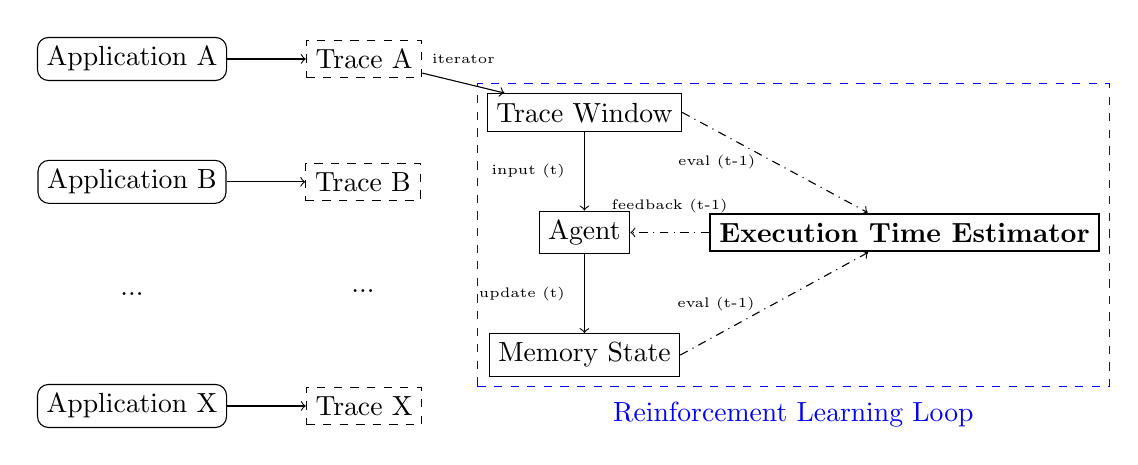
\begin{tikzpicture}[
    app/.style={rectangle, draw=black, rounded corners},
    trace/.style={rectangle, draw=black, dashed},
    env/.style={align=center, draw=blue, dashed},
    box/.style={draw=black}
  ]

  \node[app] (app0) {Application A};
  \node[app] (app1) [below=of app0] {Application B};
  \node[] (app2) [below=of app1] {...};
  \node[app] (app3) [below=of app2] {Application X};

  \node[trace] (t0) [right=of app0] {Trace A};
  \node[trace] (t1) [right=of app1] {Trace B};
  \node[] (t2) [below=of t1] {...};
  \node[trace] (t3) [right=of app3] {Trace X};
  \node[fit=(app0) (app3) (t0) (t3)] (d0) {};

  \draw[->] (app0) -- (t0);
  \draw[->] (app1) -- (t1);
  \draw[->] (app3) -- (t3);

  \node[box, xshift=10pt] (agent) [right=of d0] {Agent};
  \node[box] (window) [above=of agent] {Trace Window};
  \node[box] (memory) [below=of agent] {Memory State};
  \node[box, thick] (estimator) [right=of agent] {\textbf{Execution Time Estimator}};
  \node[env, fit=(window) (agent) (memory) (estimator)] (d1) {};
  \node[yshift=-1em] at (d1.south) {\color{blue}{Reinforcement Learning Loop}};

  \draw[->] (t0) -- (window) node [midway, label=above:{\tiny{iterator}}] {};

  \draw[->] (window) -- (agent) node [midway, label=left:{\tiny{input (t)}}] {};
  \draw[->] (agent) -- (memory) node [midway, label=left:{\tiny{update (t)}}] {};
  \draw[->, dash dot] (estimator) -- (agent) node [midway, label=above:{\tiny{feedback (t-1)}}] {};
  \draw[->, dash dot] (window.east) -- (estimator) node [midway, label=left:{\tiny{eval (t-1)}}] {};
  \draw[->, dash dot] (memory.east) -- (estimator) node [midway, label=left:{\tiny{eval (t-1)}}] {};
  
\end{tikzpicture}
\end{document}
